% Build: cd report && latexmk -xelatex report.tex   (numbers come from generated/numbers.tex)
\documentclass[10pt,a4paper]{article}
\usepackage[margin=0.9in]{geometry}
\usepackage{fontspec}
\usepackage{booktabs}
\usepackage{longtable}
\usepackage{amsmath}
\usepackage{enumitem}
\usepackage{graphicx}
\usepackage{caption}
\usepackage[numbers,sort&compress]{natbib}
\usepackage[colorlinks=true,linkcolor=black,urlcolor=blue,citecolor=black]{hyperref}
\newfontfamily\hindifont[Script=Devanagari]{Noto Sans Devanagari}
\newcommand{\hi}[1]{{\hindifont #1}}
\setlist[itemize]{leftmargin=1.3em,itemsep=0.1em,topsep=0.2em}
\setlist[enumerate]{leftmargin=1.6em,itemsep=0.1em,topsep=0.2em}
\setlength{\parskip}{0.4em}
\setlength{\parindent}{0pt}
\emergencystretch=3em
\captionsetup{font=small,labelfont=bf}
% Generated by scripts/make_report_assets.py. Do not edit.
\newcommand{\NRuns}{440}
\newcommand{\NGateCells}{66}
\newcommand{\NStrict}{43}
\newcommand{\NFirstToken}{1}
\newcommand{\NFail}{22}
\newcommand{\NCore}{24}
\newcommand{\HOnePass}{22}
\newcommand{\HOneAbove}{18}
\newcommand{\HOneMissA}{0.86}
\newcommand{\HOneMissB}{0.88}
\newcommand{\HOneMin}{0.86}
\newcommand{\HOneMedian}{0.975}
\newcommand{\HTwoNeg}{2}
\newcommand{\HThreeDiff}{+0.009}
\newcommand{\HThreeLoNinety}{-0.014}
\newcommand{\HThreeHiNinety}{+0.034}
\newcommand{\HThreeLo}{-0.017}
\newcommand{\HThreeHi}{+0.040}
\newcommand{\HFourFert}{-0.51}
\newcommand{\HFourFertLo}{-0.73}
\newcommand{\HFourFertHi}{-0.15}
\newcommand{\HFourLD}{+0.45}
\newcommand{\HFourLDLo}{+0.07}
\newcommand{\HFourLDHi}{+0.72}
\newcommand{\HFiveMLPGain}{-0.05}
\newcommand{\HFiveMLPLo}{-0.21}
\newcommand{\HFiveMLPHi}{+0.10}
\newcommand{\HFiveHeadGain}{-0.36}
\newcommand{\HFiveHeadLo}{-0.39}
\newcommand{\HFiveHeadHi}{-0.32}
\newcommand{\CostEAP}{3.5}
\newcommand{\CostAP}{49}
\newcommand{\MeanTAP}{157}
\newcommand{\MeanTAttr}{3.2}
\newcommand{\NTimed}{120}
\newcommand{\SweepA}{0.59}
\newcommand{\SweepB}{0.58}
\newcommand{\SweepC}{0.59}
\newcommand{\NoisingRho}{0.93}
\newcommand{\HindiFailLo}{0.27}
\newcommand{\HindiFailHi}{0.64}
\newcommand{\HindiFailN}{17}
\newcommand{\GPTRho}{0.99}
\newcommand{\GPTEapRho}{0.40}
\newcommand{\GPTMlpAttr}{-0.93}
\newcommand{\GPTMlpEap}{+0.95}
\newcommand{\GPTLayerZeroAP}{0.88}
\newcommand{\GPTLayerZeroAttr}{-0.46}
\newcommand{\QwenMlpAttr}{-0.87}
\newcommand{\BloomMlpLo}{0.997}
\newcommand{\BloomMlpHi}{0.998}
\newcommand{\HFiveHeadGainCheck}{-0.36}


\newcommand{\AP}{\mathrm{AP}}
\newcommand{\AttrP}{\mathrm{AttrP}}

\title{When does attribution patching agree with activation patching\\ across tasks and languages?}
\author{Hrishiraj Mitra (2023111037)\\ CL3.412 Mechanistic Interpretability of Language Models, IIIT Hyderabad}
\date{November 2026}

\begin{document}
\maketitle

\begin{abstract}
Activation patching (AP) is the standard causal test for which attention heads and MLPs a language model uses for a behaviour, but it needs one forward pass per component. Attribution patching (AttrP) replaces those passes with one gradient. It is only useful where it ranks components the way AP does, and that has mostly been checked in English on a few tasks. I compare AP, first-order AttrP and a node-level integrated-gradients variant (EAP-IG) on \NRuns{} runs: nine models of at most 2B parameters, four tasks, English and Hindi, both patching directions, five prompt seeds. A competence gate decides first whether a model does the task at all. Of \NGateCells{} candidate cells, \NStrict{} pass strictly and \NFail{} fail; every Hindi IOI cell fails, because the models cannot do the task. Where the comparison can be run, AttrP reproduces the AP head ranking in \HOnePass{} of 24 core cells (Spearman $\rho\ge0.90$) at about $1/\CostAP$ of the cost. For the one task where Hindi can be tested well (agreement, BLOOM), Hindi agrees as well as English, within $\pm0.05$. AttrP fails on MLP outputs of IOI-type circuits, and this failure sits in MLP layer~0. EAP-IG repairs layer~0 on GPT-2 IOI but lowers head agreement by \HFiveHeadGain{} on average, so it is not a free upgrade. The Hindi evidence rests on one task and one model family.
\end{abstract}

\section{Introduction}
Mechanistic interpretability asks which components of a network implement a behaviour. Activation patching answers it causally: copy one component's activation from a run where the model behaves correctly (clean) into a run where it does not (corrupted), and measure how much of the behaviour is restored \citep{heimersheim2024patching,zhang2023bestpractices}. The cost is one forward pass per component, which becomes impractical for large models. Attribution patching approximates the same quantity with a first-order Taylor expansion, needing one backward pass for all components at once \citep{nanda2023attribution,syed2023attribution}. Prior work already shows it is weak in some places: it can miss components when attention saturates or when effects cancel \citep{kramar2024atp}, and Nanda's write-up notes it is less reliable in early layers.

This project asks where the approximation holds once the \emph{task}, the \emph{language} and the \emph{model} change. A running example is subject--verb agreement scored on the next token (Table~\ref{tab:tasks}); the Hindi version is
\begin{center}\small
\hi{चैनल भविष्य में ऐसी घटना की पुनरावृत्ति नहीं होने का वचन देता} \;\textbf{\hi{है}} vs.\ \hi{हों}\quad
\textit{(`The channel promises that such an incident will not recur': is.3SG vs.\ be.3PL)}
\end{center}
\textbf{Contributions.} (i) A controlled comparison of AP, AttrP and EAP-IG over a model $\times$ task $\times$ language grid, run only where a model passes a competence gate. (ii) The gate itself yields a result: most small multilingual models cannot do the Hindi tasks, which limits what can be compared. (iii) To my knowledge, a first check of whether attribution patching holds in a language other than English; it does, within a margin fixed in advance, on agreement in the BLOOM family. (iv) Two refinements of known caveats: the MLP disagreement is concentrated in layer~0, and integrated gradients at node level trades MLP agreement for head agreement. The general advice ``use attribution patching as a cheap first pass and verify with real patching'' is not new; this study tests it across more settings.

\section{Method}
\subsection{Tasks, corruptions and metric}
\begin{table}[h]
\centering\small
\begin{tabular}{@{}lp{5.6cm}p{4.3cm}p{2.2cm}@{}}
\toprule
Task & Clean prompt, answer pair & Corrupted prompt & Languages\\
\midrule
IOI & name-swap sentence; IO vs.\ S name & all three names replaced (ABC) & en, hi, romanised hi\\
Capitals & ``The capital of $X$ is'' & a different country & en, hi\\
Agreement & MultiBLiMP prefix; agreeing vs.\ non-agreeing verb \citep{jumelet2025multiblimp} & prefix of another example, equal length & en, hi\\
Induction & $\dots$ A B $\dots$ A $\to$ B & repeat broken & en, hi\\
\bottomrule
\end{tabular}
\caption{Tasks. Clean and corrupted prompts always have equal token length, so no padding is used. The metric is the logit difference $m=\mathrm{logit}(y^+)-\mathrm{logit}(y^-)$ at the last position.}
\label{tab:tasks}
\end{table}
IOI follows \citet{wang2022ioi} and uses the ABC corruption as primary. Hindi IOI templates end before the recipient, because Hindi is verb-final.

\subsection{Models and the competence gate}
Nine models fit one 11\,GB GPU in fp32: GPT-2 small (anchor), Pythia-160m and 410m \citep{biderman2023pythia} (English controls), Qwen2.5-0.5B and 1.5B \citep{qwen2024qwen25}, Llama-3.2-1B \citep{llama2024herd} and BLOOM-560m, 1b1 and 1b7 \citep{workshop2022bloom}, all through TransformerLens 2.15 \citep{nanda2022transformerlens}. Gemma-3-1B was planned but TransformerLens 2.15 cannot load it, so BLOOM, which has Hindi in its pretraining data, replaced it; Sarvam-1 (Indic-focused, optional) was dropped for the same reason.

Agreement between two methods is meaningless if the model does not do the task, so every (model, task, language) cell is first screened on 100 prompts (seed 0). A cell passes only if clean accuracy $\ge0.80$, mean clean logit difference $\ge0.5$, corrupted logit difference $\le\max(0.25,\,0.5\times\text{clean})$, and at least 90\% of answers are single tokens. Cells failing only the last criterion form a \emph{first-token tier}, run for sensitivity but excluded from the hypothesis tests. The gate stays fixed for all analyses.

\subsection{Three attribution methods}
Let $a_c$ be the output of component $c$ (one attention head's \texttt{hook\_z}, or one MLP output). In the denoising direction the target is the corrupted run and the source is the clean run.
\begin{align}
\Delta_c^{\AP} &= \frac{m(\text{corr}\mid a_c\leftarrow a_c^{\text{clean}})-m(\text{corr})}{m(\text{clean})-m(\text{corr})},\\
\Delta_c^{\AttrP} &= \frac{(a_c^{\text{clean}}-a_c^{\text{corr}})\cdot\nabla_{a_c}m\,\big|_{\text{corr}}}{m(\text{clean})-m(\text{corr})},\\
\Delta_c^{\text{EAP-IG}} &= \frac{(a_c^{\text{clean}}-a_c^{\text{corr}})\cdot\frac1n\sum_{k=1}^{n}\nabla_{a_c}m\,\big|_{x(\alpha_k)}}{m(\text{clean})-m(\text{corr})},
\end{align}
with $x(\alpha)=e^{\text{corr}}+\alpha(e^{\text{clean}}-e^{\text{corr}})$ in token-embedding space and $\alpha_k=(k+\tfrac12)/n$. The noising direction swaps the roles. AP is exact but costs one pass per component; AttrP costs one forward and one backward pass in total; EAP-IG costs $n$ of each. I use $n=5$ and sweep $n\in\{5,10,20\}$ on seed 0. This EAP-IG is \emph{node-level}, not the edge-level method of \citet{hanna2024faith}. Weights are frozen and everything runs in fp32. Each run checks its fast AP path (starting at the patched layer) against the full forward pass, and EAP-IG with the single step $\alpha=0$ equals AttrP exactly (checked on GPT-2, both directions).

\subsection{Agreement metrics and hypotheses}
For each cell: head Spearman $\rho(\Delta^{\AP},\Delta^{\AttrP})$ over all heads; a restricted $\rho$ over heads with $|\Delta^{\AP}|>0.05$ (fixed in advance because most heads have near-zero effect); top-$k$ overlap of the $k$ heads with largest $|\Delta|$, $k=14$ primary; MLP Pearson $r$ over layers; wall-clock cost. A cell is GO if $\rho\ge0.90$ and top-14 overlap $\ge0.5$. Each cell uses five seeds that resample the 100 prompts; confidence intervals are over seeds or cells, so they describe prompt sampling, not variation across trained models. The five hypotheses, fixed before the grid (Section~\ref{sec:dev} lists every deviation):
\begin{itemize}
\item[\textbf{H1}] head $\rho\ge0.90$ in every core cell;
\item[\textbf{H2}] MLP $r(\AP,\AttrP)<0$ in a majority of core cells;
\item[\textbf{H3}] AttrP agrees less in Hindi than in English on matched (model, task) pairs, tested by a paired bootstrap and by equivalence (TOST, margin $\pm0.05$, 90\% CI);
\item[\textbf{H4}] $\rho$ falls with tokenizer fertility and rises with clean logit difference (observational);
\item[\textbf{H5}] EAP-IG gives higher MLP agreement than AttrP and is worth its cost.
\end{itemize}
``Core'' cells are the strict-pass cells for GPT-2, Qwen2.5, Llama-3.2 and BLOOM on IOI, capitals and agreement (24 cells). Pythia and induction are an English robustness appendix.

\section{Results}
\subsection{Gate coverage}
\begin{figure}[t]
\centering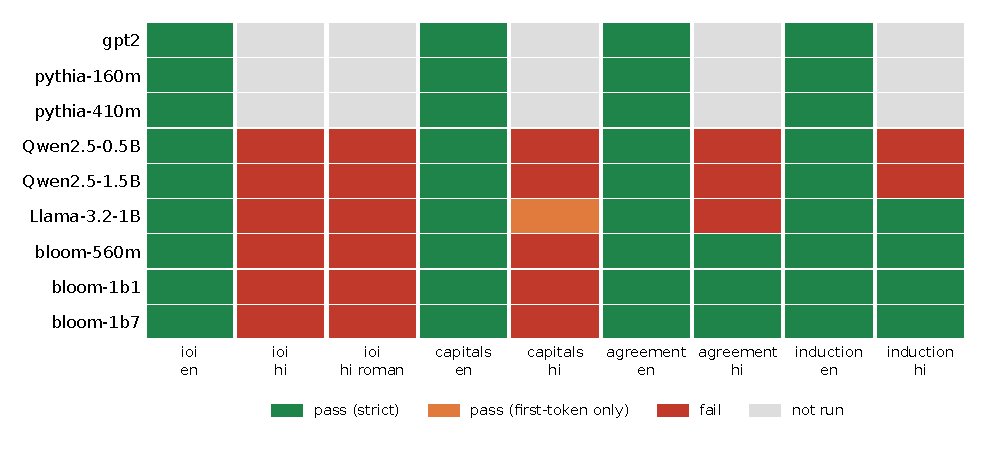
\includegraphics[width=0.92\textwidth]{generated/fig_gate.pdf}
\caption{Competence gate over \NGateCells{} candidate cells. English passes almost everywhere. Hindi passes only for agreement on BLOOM and for induction on BLOOM and Llama.}
\label{fig:gate}
\end{figure}
\NStrict{} cells pass strictly, \NFirstToken{} passes only in the first-token tier (Llama-3.2-1B capitals, Hindi) and \NFail{} fail (Figure~\ref{fig:gate}; full table in Appendix~\ref{app:gate}). Hindi IOI and romanised-Hindi IOI fail in every model. Across the \HindiFailN{} failing Hindi IOI, capitals and romanised cells, clean accuracy is between \HindiFailLo{} and \HindiFailHi{}, so the models cannot do the task and there is nothing to localise. Qwen2.5 and Llama cannot form a single-token Hindi agreement contrast at all: with byte-level BPE the first token of the correct and incorrect verb form coincide. Hindi IOI templates were read by one native speaker (the author) after the grid ran; one place word was corrected and the Hindi gate re-run, with no status change.

\subsection{H1: head rankings agree}
\begin{figure}[t]
\centering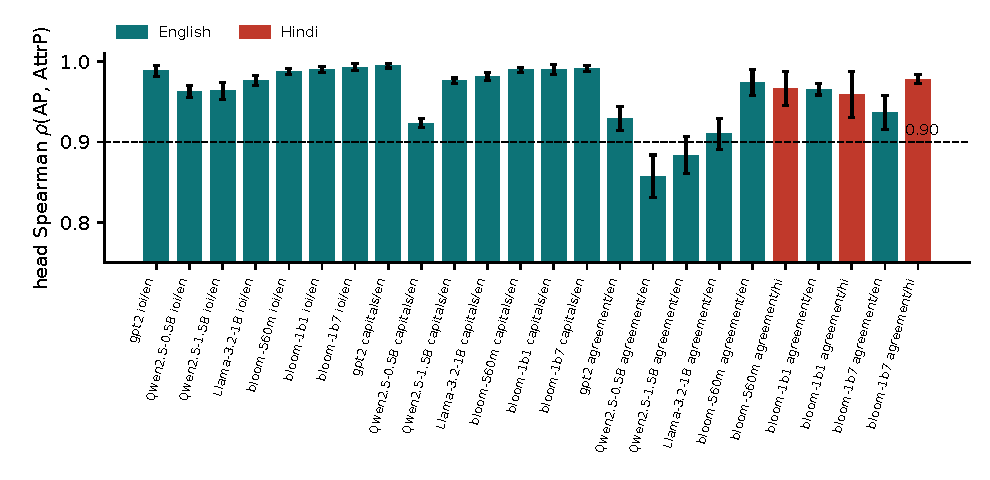
\includegraphics[width=\textwidth]{generated/fig_rho_cells.pdf}
\caption{Head Spearman $\rho$(AP, AttrP) per core cell (mean $\pm$ sd over five seeds, denoising). Dashed line: the 0.90 bar.}
\label{fig:rho}
\end{figure}
Head agreement meets the bar in \HOnePass{} of 24 core cells and exceeds 0.95 in \HOneAbove{} (Figure~\ref{fig:rho}, Appendix Table~\ref{tab:cells}). The two misses are both Qwen2.5 on English agreement ($\rho=\HOneMissA$ and $\HOneMissB$). H1 as stated (every cell) therefore does not hold, but the exception is small: the lowest cell is \HOneMin{}. The noising direction is somewhat lower (mean $\rho=\NoisingRho$; Qwen and Llama agreement 0.76--0.86; Appendix Table~\ref{tab:noise}). AP costs about \CostAP$\times$ AttrP in wall time (median per-run ratio over \NTimed{} core denoising runs; means \MeanTAP\,s versus \MeanTAttr\,s).

\subsection{H3: Hindi is as good as English where it can be tested}
\begin{figure}[t]
\centering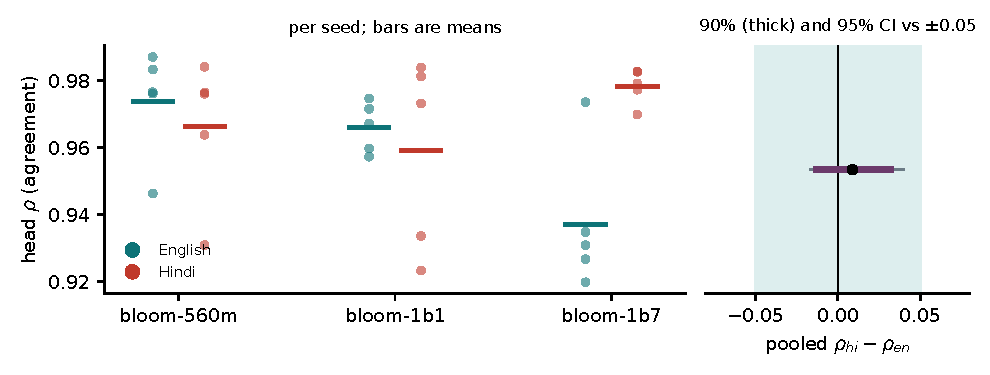
\includegraphics[width=\textwidth]{generated/fig_hindi.pdf}
\caption{Agreement task on BLOOM. Left: head $\rho$ per seed, English and Hindi. Right: pooled Hindi-minus-English difference with its 90\% and 95\% intervals against the $\pm0.05$ equivalence margin.}
\label{fig:hindi}
\end{figure}
Only BLOOM-560m, 1b1 and 1b7 pass the gate for agreement in both languages. The Hindi-minus-English difference in $\rho$ is $-0.008$, $-0.007$ and $+0.041$; pooled it is \HThreeDiff{} with 90\% CI [\HThreeLoNinety, \HThreeHiNinety] and 95\% CI [\HThreeLo, \HThreeHi]. The 90\% interval lies inside $\pm0.05$, so AttrP is equivalent in the two languages within the margin fixed in advance (Figure~\ref{fig:hindi}); H3 is not supported. \textbf{Scope:} one task, one family, three pairs. The expected way for Hindi to break the approximation was tokenisation, since Hindi words split into more tokens; it did not break here, but this says nothing about Hindi IOI or factual recall, where no model passed the gate.

\subsection{H2 and the layer-0 failure}
\begin{figure}[t]
\centering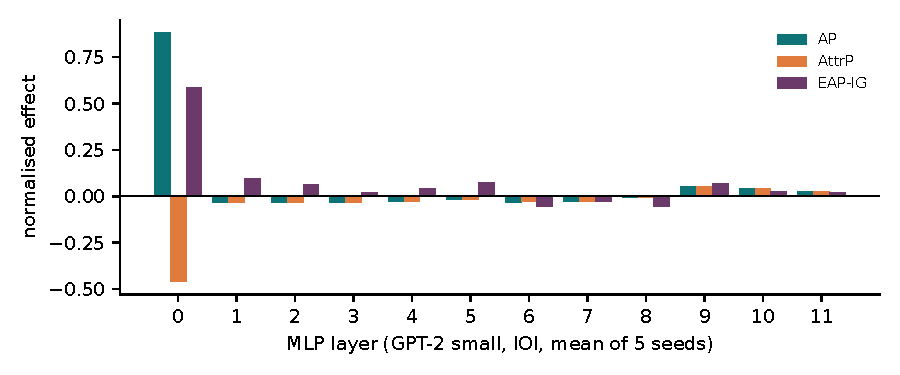
\includegraphics[width=0.78\textwidth]{generated/fig_mlp_layers.pdf}
\caption{GPT-2 small, IOI: normalised effect of each MLP layer under AP, AttrP and EAP-IG. Layer 0 is where AP and AttrP disagree; the remaining layers match.}
\label{fig:mlp}
\end{figure}
MLP agreement is negative in only \HTwoNeg{} of 24 cells, so H2 is rejected as a general claim. The pilot failure on GPT-2 IOI ($r=\GPTMlpAttr$) reproduces in Qwen2.5-0.5B IOI ($r=\QwenMlpAttr$) and in Pythia IOI and induction, but BLOOM IOI agrees almost perfectly ($r>0.99$). The failure is circuit-specific, not general. On GPT-2 IOI the MLP disagreement is concentrated in layer~0: AP gives \GPTLayerZeroAP{}, AttrP gives \GPTLayerZeroAttr{} (Figure~\ref{fig:mlp}). This localisation is a post hoc observation across GPT-2, Qwen2.5-0.5B and the Pythias, and it is consistent with the known weakness of the first-order approximation where activations change a lot, as in early layers acting as an extended embedding.

\subsection{H5: integrated gradients is not a free upgrade}
\begin{figure}[t]
\centering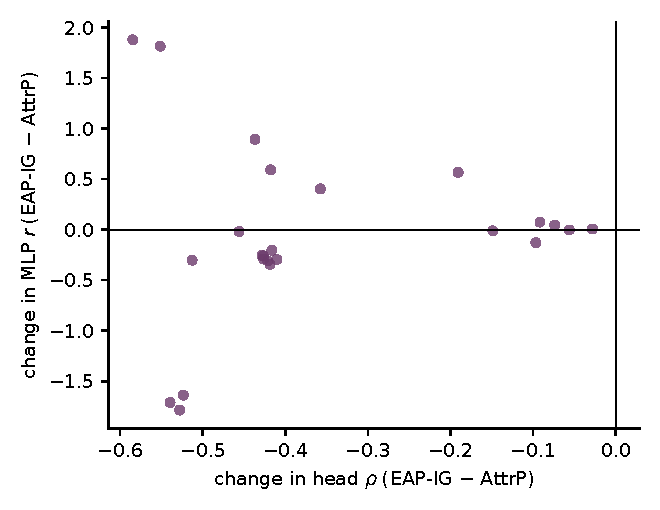
\includegraphics[width=0.55\textwidth]{generated/fig_eap_tradeoff.pdf}
\caption{Per core cell: change in MLP $r$ against change in head $\rho$ when moving from AttrP to EAP-IG (5 steps, denoising). Every core cell loses head agreement; MLP agreement rises in some cells and falls in others.}
\label{fig:eap}
\end{figure}
Pooled over core cells, EAP-IG changes MLP agreement by \HFiveMLPGain{} (95\% CI [\HFiveMLPLo, \HFiveMLPHi]) and changes head agreement by \HFiveHeadGain{} (CI [\HFiveHeadLo, \HFiveHeadHi]), at about \CostEAP$\times$ the cost of AttrP. H5 is rejected. Convergence is not the explanation: mean head $\rho$ is \SweepA{}, \SweepB{} and \SweepC{} at 5, 10 and 20 steps. On GPT-2 IOI specifically, EAP-IG does repair layer~0 (MLP $r$ \GPTMlpAttr{} $\to$ \GPTMlpEap{}) while head $\rho$ falls from \GPTRho{} to \GPTEapRho{} (exploratory). A plausible reason is that along the integration path every component moves toward its clean value at once, whereas AP moves one component and holds the rest corrupted, so EAP-IG answers a slightly different question. I did not test that explanation, and this node-level variant should not be read as a result about Hanna et al.'s edge-level method.

\subsection{H4: fertility and logit difference}
Across the 24 core cells, Spearman $\rho$ between agreement and tokens per word is \HFourFert{} (95\% CI [\HFourFertLo, \HFourFertHi]) and between agreement and clean logit difference is \HFourLD{} (CI [\HFourLDLo, \HFourLDHi]). The signs match H4, but fertility is entangled with model and task, and no Hindi cell with high fertility passed the gate, so this does not show a causal effect of Hindi.

\section{Discussion}
\textbf{What to do in practice.} Within this grid, a gradient pass is a good first screen for \emph{which heads matter}: it recovers the AP ranking in nearly all gated cells at about 2\% of the cost. It should not be trusted for MLP outputs of IOI-type circuits, and layer~0 is where to check first with real patching. Switching to node-level integrated gradients is not a safe default.

\textbf{Relation to prior work.} \citet{syed2023attribution} report a weak attribution-versus-activation correlation for edges on a different task, and \citet{kramar2024atp} document false negatives from attention saturation and cancellation. My high rank agreement does not contradict these: I score head and MLP outputs with a rank statistic on tasks with a few dominant components, and I did not test attention-pattern patching, the saturation case. I do not interpret the restricted $\rho$ (heads with $|\Delta^{\AP}|>0.05$): in many cells only a handful of heads pass the cut-off, so it rests on very few points (Appendix Table~\ref{tab:cells}).

\section{Limitations and deviations from the preregistration}\label{sec:dev}
\begin{enumerate}
\item \textbf{Narrow Hindi evidence.} Testable Hindi cells are agreement and induction on BLOOM and induction on Llama. Nothing is claimed for Hindi IOI, factual recall, or script versus language. This is a limit of the models, and is itself the main finding about Hindi.
\item \textbf{H3 has three pairs from one family.} English agreement windows are shorter (about 7 tokens of context) than Hindi (about 23), so sequence length is a confound for H3 and H4.
\item \textbf{Seeds resample prompts, not models.} Intervals reflect prompt sampling only.
\item \textbf{Single-token agreement pool.} Agreement uses MultiBLiMP pairs with one-token answers, which selects frequent verbs.
\item \textbf{Gate changes after seeing gate numbers, before any patching result} (Amendment 2): the corrupted-logit-difference rule gained the ``or $\le0.5\times$ clean'' branch (agreement and induction corruptions leave a residual grammatical preference, and the fixed cap rejected every agreement cell); the first-token tier was introduced; BLOOM-1b1 and 1b7 were added because the first gate left a single strict Hindi cell; Gemma-3 was replaced by BLOOM.
\item \textbf{The 0.90 head bar is a judgement call.} The v1 pilot used 0.80 and reached about 0.99. At 0.80 every core cell would pass; both Qwen misses (0.86, 0.88) are above it. The restricted-$\rho$ cut-off of 0.05 came from the pilot's exploratory analysis. The layer-0 localisation and the GPT-2 EAP-IG trade-off are exploratory.
\item \textbf{Bugs found by the checks and fixed before the grid:} noising-direction AttrP and EAP-IG had the opposite sign to AP; MultiBLiMP contrasts contained contractions and glued punctuation; the capitals answer pool had multi-token answers.
\item \textbf{One reviewer.} The Hindi templates were checked by one native speaker, the author, after the grid, with no independent second reviewer.
\item \textbf{Model provenance.} Llama-3.2-1B weights come from the ungated \texttt{unsloth} mirror because the official repository refused the access token. Models are at most 2B parameters; nothing is claimed above that.
\end{enumerate}

\section{Reproducibility}
Code and results: \url{https://github.com/hrishirajmitra/attrp-ap-hindi}. The repository holds all code, per-run results (\texttt{results/grid/}, 440 runs), the gate output and the analysis tables are in the project repository; the protocol is in \texttt{PREREGISTRATION\_v2.md} with its amendments and the numbers quoted here are generated from \texttt{results/analysis/summary.json} and \texttt{cells.csv} by \texttt{scripts/make\_report\_assets.py}. Runs used one RTX 2080 Ti per job on the university cluster, about 4 hours wall-clock on up to 12 GPUs for the whole grid. A GPT-2 IOI pilot (v1, five seeds) preceded the grid: AttrP head $\rho=0.99$ and MLP $r=-0.93$ under ABC corruption.

\bibliographystyle{plainnat}
\bibliography{references}

\clearpage
\appendix
\section{Full gate table}\label{app:gate}
{\small
\begin{longtable}{@{}lllrrrl@{}}
\toprule
Model & Task & Lang & Acc. & Clean LD & 1-token & Tier\\
\midrule
\endhead
\bottomrule
\endlastfoot
gpt2 & ioi & en & 0.99 & 3.15 & 1.00 & strict \\
gpt2 & capitals & en & 0.99 & 5.00 & 1.00 & strict \\
gpt2 & agreement & en & 0.88 & 3.18 & 1.00 & strict \\
gpt2 & induction & en & 0.86 & 2.23 & 1.00 & strict \\
pythia-160m & ioi & en & 0.94 & 4.91 & 1.00 & strict \\
pythia-160m & capitals & en & 1.00 & 4.43 & 1.00 & strict \\
pythia-160m & agreement & en & 0.82 & 2.59 & 1.00 & strict \\
pythia-160m & induction & en & 0.88 & 1.92 & 1.00 & strict \\
pythia-410m & ioi & en & 1.00 & 4.33 & 1.00 & strict \\
pythia-410m & capitals & en & 1.00 & 7.62 & 1.00 & strict \\
pythia-410m & agreement & en & 0.83 & 3.36 & 1.00 & strict \\
pythia-410m & induction & en & 0.92 & 2.65 & 1.00 & strict \\
Qwen2.5-0.5B & ioi & en & 1.00 & 5.76 & 1.00 & strict \\
Qwen2.5-0.5B & ioi & hi & 0.30 & 0.01 & 0.00 & fail \\
Qwen2.5-0.5B & ioi & hi\_roman & 0.50 & -0.08 & 0.00 & fail \\
Qwen2.5-0.5B & capitals & en & 1.00 & 9.40 & 1.00 & strict \\
Qwen2.5-0.5B & capitals & hi & 0.48 & -0.13 & 0.00 & fail \\
Qwen2.5-0.5B & agreement & en & 0.83 & 3.45 & 1.00 & strict \\
Qwen2.5-0.5B & agreement & hi & -- & -- & -- & fail \\
Qwen2.5-0.5B & induction & en & 0.96 & 3.48 & 1.00 & strict \\
Qwen2.5-0.5B & induction & hi & 0.62 & 0.69 & 1.00 & fail \\
Qwen2.5-1.5B & ioi & en & 0.97 & 5.18 & 1.00 & strict \\
Qwen2.5-1.5B & ioi & hi & 0.27 & -0.01 & 0.00 & fail \\
Qwen2.5-1.5B & ioi & hi\_roman & 0.45 & -0.02 & 0.00 & fail \\
Qwen2.5-1.5B & capitals & en & 1.00 & 10.78 & 1.00 & strict \\
Qwen2.5-1.5B & capitals & hi & 0.46 & -0.15 & 0.00 & fail \\
Qwen2.5-1.5B & agreement & en & 0.87 & 3.85 & 1.00 & strict \\
Qwen2.5-1.5B & agreement & hi & -- & -- & -- & fail \\
Qwen2.5-1.5B & induction & en & 0.94 & 3.91 & 1.00 & strict \\
Qwen2.5-1.5B & induction & hi & 0.75 & 1.21 & 1.00 & fail \\
Llama-3.2-1B & ioi & en & 1.00 & 5.04 & 1.00 & strict \\
Llama-3.2-1B & ioi & hi & 0.32 & -1.18 & 0.00 & fail \\
Llama-3.2-1B & ioi & hi\_roman & 0.60 & 0.43 & 0.00 & fail \\
Llama-3.2-1B & capitals & en & 1.00 & 10.95 & 1.00 & strict \\
Llama-3.2-1B & capitals & hi & 0.91 & 3.22 & 0.00 & first-token \\
Llama-3.2-1B & agreement & en & 0.92 & 3.31 & 1.00 & strict \\
Llama-3.2-1B & agreement & hi & 0.69 & 1.32 & 0.02 & fail \\
Llama-3.2-1B & induction & en & 0.91 & 3.51 & 1.00 & strict \\
Llama-3.2-1B & induction & hi & 0.99 & 3.78 & 1.00 & strict \\
bloom-560m & ioi & en & 1.00 & 4.72 & 1.00 & strict \\
bloom-560m & ioi & hi & 0.54 & 0.34 & 1.00 & fail \\
bloom-560m & ioi & hi\_roman & 0.40 & -0.29 & 0.00 & fail \\
bloom-560m & capitals & en & 0.94 & 7.70 & 1.00 & strict \\
bloom-560m & capitals & hi & 0.51 & 0.05 & 0.00 & fail \\
bloom-560m & agreement & en & 0.87 & 3.26 & 1.00 & strict \\
bloom-560m & agreement & hi & 0.90 & 4.79 & 1.00 & strict \\
bloom-560m & induction & en & 0.99 & 4.16 & 1.00 & strict \\
bloom-560m & induction & hi & 0.98 & 3.10 & 1.00 & strict \\
bloom-1b1 & ioi & en & 1.00 & 4.07 & 1.00 & strict \\
bloom-1b1 & ioi & hi & 0.56 & 0.27 & 1.00 & fail \\
bloom-1b1 & ioi & hi\_roman & 0.30 & -0.93 & 0.00 & fail \\
bloom-1b1 & capitals & en & 1.00 & 10.22 & 1.00 & strict \\
bloom-1b1 & capitals & hi & 0.63 & 0.73 & 0.00 & fail \\
bloom-1b1 & agreement & en & 0.83 & 3.34 & 1.00 & strict \\
bloom-1b1 & agreement & hi & 0.90 & 4.78 & 1.00 & strict \\
bloom-1b1 & induction & en & 0.97 & 3.93 & 1.00 & strict \\
bloom-1b1 & induction & hi & 0.92 & 2.02 & 1.00 & strict \\
bloom-1b7 & ioi & en & 1.00 & 3.12 & 1.00 & strict \\
bloom-1b7 & ioi & hi & 0.64 & 0.56 & 1.00 & fail \\
bloom-1b7 & ioi & hi\_roman & 0.33 & -0.70 & 0.00 & fail \\
bloom-1b7 & capitals & en & 1.00 & 10.14 & 1.00 & strict \\
bloom-1b7 & capitals & hi & 0.58 & 0.33 & 0.00 & fail \\
bloom-1b7 & agreement & en & 0.84 & 3.36 & 1.00 & strict \\
bloom-1b7 & agreement & hi & 0.91 & 5.17 & 1.00 & strict \\
bloom-1b7 & induction & en & 0.98 & 4.21 & 1.00 & strict \\
bloom-1b7 & induction & hi & 0.91 & 2.16 & 1.00 & strict
\\
\end{longtable}}

\section{Per-cell agreement}
\begin{table}[h]
\centering\small
\setlength{\tabcolsep}{4pt}
\begin{tabular}{@{}lllcccccc@{}}
\toprule
Model & Task & Lang & $\rho$ (mean $\pm$ sd) & restr.\ $\rho$ & top-14 & MLP $r$ & EAP $\rho$ & EAP MLP $r$\\
\midrule
gpt2 & ioi & en & 0.989 $\pm$ 0.007 & 1.00 & 0.99 & -0.93 & 0.40 & +0.95 \\
gpt2 & capitals & en & 0.995 $\pm$ 0.003 & 1.00 & 0.97 & +0.99 & 0.97 & +1.00 \\
gpt2 & agreement & en & 0.930 $\pm$ 0.015 & 0.75 & 0.83 & +0.25 & 0.51 & +0.84 \\
Qwen2.5-0.5B & ioi & en & 0.963 $\pm$ 0.008 & 1.00 & 1.00 & -0.87 & 0.41 & +0.95 \\
Qwen2.5-0.5B & capitals & en & 0.924 $\pm$ 0.006 & 1.00 & 0.83 & +0.91 & 0.83 & +0.99 \\
Qwen2.5-0.5B & agreement & en & 0.858 $\pm$ 0.026 & 1.00 & 0.60 & +0.54 & 0.50 & +0.95 \\
Qwen2.5-1.5B & ioi & en & 0.964 $\pm$ 0.010 & 0.94 & 0.94 & +0.98 & 0.45 & +0.68 \\
Qwen2.5-1.5B & capitals & en & 0.977 $\pm$ 0.003 & 0.96 & 0.83 & +0.91 & 0.83 & +0.89 \\
Qwen2.5-1.5B & agreement & en & 0.884 $\pm$ 0.023 & 0.90 & 0.71 & +0.81 & 0.47 & +0.46 \\
Llama-3.2-1B & ioi & en & 0.977 $\pm$ 0.007 & 0.93 & 0.86 & +0.06 & 0.54 & +0.95 \\
Llama-3.2-1B & capitals & en & 0.982 $\pm$ 0.005 & 0.96 & 0.93 & +0.37 & 0.79 & +0.93 \\
Llama-3.2-1B & agreement & en & 0.910 $\pm$ 0.019 & 1.00 & 0.83 & +0.85 & 0.45 & +0.83 \\
bloom-560m & ioi & en & 0.988 $\pm$ 0.004 & 1.00 & 0.97 & +1.00 & 0.46 & -0.64 \\
bloom-560m & capitals & en & 0.990 $\pm$ 0.003 & 0.84 & 0.99 & +0.90 & 0.92 & +0.94 \\
bloom-560m & agreement & en & 0.974 $\pm$ 0.016 & 0.75 & 0.94 & +0.98 & 0.55 & +0.73 \\
bloom-560m & agreement & hi & 0.966 $\pm$ 0.021 & 1.00 & 0.89 & +0.98 & 0.54 & +0.67 \\
bloom-1b1 & ioi & en & 0.990 $\pm$ 0.004 & 1.00 & 1.00 & +1.00 & 0.46 & -0.79 \\
bloom-1b1 & capitals & en & 0.990 $\pm$ 0.006 & 0.86 & 1.00 & +0.89 & 0.93 & +0.89 \\
bloom-1b1 & agreement & en & 0.966 $\pm$ 0.007 & 0.75 & 0.86 & +0.96 & 0.54 & +0.70 \\
bloom-1b1 & agreement & hi & 0.959 $\pm$ 0.028 & -- & 0.93 & +0.96 & 0.55 & +0.67 \\
bloom-1b7 & ioi & en & 0.993 $\pm$ 0.004 & 1.00 & 1.00 & +1.00 & 0.45 & -0.71 \\
bloom-1b7 & capitals & en & 0.992 $\pm$ 0.004 & 0.98 & 1.00 & +0.95 & 0.89 & +0.83 \\
bloom-1b7 & agreement & en & 0.937 $\pm$ 0.021 & 0.75 & 0.81 & +0.98 & 0.52 & +0.78 \\
bloom-1b7 & agreement & hi & 0.978 $\pm$ 0.005 & -- & 1.00 & +0.99 & 0.55 & +0.70
\\
\bottomrule
\end{tabular}
\caption{Core cells, denoising, mean over five seeds. Restricted $\rho$ (heads with $|\Delta^{\AP}|>0.05$) is ``--'' where fewer than three heads qualify and rests on few heads elsewhere. ``EAP'' columns compare EAP-IG (5 steps) with AP.}
\label{tab:cells}
\end{table}

\begin{table}[h]
\centering\small
\begin{tabular}{@{}lllccc@{}}
\toprule
Model & Task & Lang & $\rho$ & top-14 & MLP $r$\\
\midrule
gpt2 & ioi & en & 0.915 & 0.83 & -0.66 \\
gpt2 & capitals & en & 0.994 & 0.99 & +0.99 \\
gpt2 & agreement & en & 0.882 & 0.67 & -0.03 \\
Qwen2.5-0.5B & ioi & en & 0.917 & 0.83 & +0.04 \\
Qwen2.5-0.5B & capitals & en & 0.919 & 0.83 & +0.92 \\
Qwen2.5-0.5B & agreement & en & 0.758 & 0.51 & +0.21 \\
Qwen2.5-1.5B & ioi & en & 0.866 & 0.87 & +0.72 \\
Qwen2.5-1.5B & capitals & en & 0.979 & 0.84 & +0.91 \\
Qwen2.5-1.5B & agreement & en & 0.833 & 0.44 & +0.14 \\
Llama-3.2-1B & ioi & en & 0.908 & 0.89 & +0.61 \\
Llama-3.2-1B & capitals & en & 0.980 & 0.96 & +0.36 \\
Llama-3.2-1B & agreement & en & 0.855 & 0.61 & -0.15 \\
bloom-560m & ioi & en & 0.958 & 0.91 & +0.92 \\
bloom-560m & capitals & en & 0.988 & 1.00 & +0.90 \\
bloom-560m & agreement & en & 0.953 & 0.84 & +0.92 \\
bloom-560m & agreement & hi & 0.933 & 0.89 & +0.44 \\
bloom-1b1 & ioi & en & 0.962 & 0.97 & +0.85 \\
bloom-1b1 & capitals & en & 0.992 & 1.00 & +0.89 \\
bloom-1b1 & agreement & en & 0.954 & 0.81 & +0.66 \\
bloom-1b1 & agreement & hi & 0.898 & 0.87 & +0.37 \\
bloom-1b7 & ioi & en & 0.984 & 0.96 & +0.87 \\
bloom-1b7 & capitals & en & 0.988 & 1.00 & +0.96 \\
bloom-1b7 & agreement & en & 0.934 & 0.87 & +0.89 \\
bloom-1b7 & agreement & hi & 0.947 & 0.87 & +0.75
\\
\bottomrule
\end{tabular}
\caption{Noising direction, core cells, mean over five seeds (AttrP versus AP).}
\label{tab:noise}
\end{table}

\begin{table}[h]
\centering\small
\begin{tabular}{@{}lllccc@{}}
\toprule
Model & Task & Lang & $\rho$ & top-14 & MLP $r$\\
\midrule
gpt2 & induction & en & 0.962 & 0.90 & -0.16 \\
pythia-160m & ioi & en & 0.951 & 0.94 & -0.89 \\
pythia-160m & capitals & en & 0.931 & 0.99 & +1.00 \\
pythia-160m & agreement & en & 0.843 & 0.73 & +0.63 \\
pythia-160m & induction & en & 0.926 & 0.93 & -0.57 \\
pythia-410m & ioi & en & 0.984 & 0.99 & -0.83 \\
pythia-410m & capitals & en & 0.983 & 0.94 & +0.97 \\
pythia-410m & agreement & en & 0.921 & 0.79 & +0.47 \\
pythia-410m & induction & en & 0.967 & 0.94 & +0.19 \\
Qwen2.5-0.5B & induction & en & 0.924 & 0.89 & +0.02 \\
Qwen2.5-1.5B & induction & en & 0.930 & 0.76 & +0.86 \\
Llama-3.2-1B & induction & en & 0.957 & 0.89 & +0.24 \\
Llama-3.2-1B & induction & hi & 0.969 & 0.93 & +0.41 \\
bloom-560m & induction & en & 0.988 & 0.94 & +0.98 \\
bloom-560m & induction & hi & 0.991 & 0.90 & +0.96 \\
bloom-1b1 & induction & en & 0.991 & 0.96 & +0.91 \\
bloom-1b1 & induction & hi & 0.995 & 1.00 & +0.90 \\
bloom-1b7 & induction & en & 0.987 & 0.94 & +0.95 \\
bloom-1b7 & induction & hi & 0.991 & 0.93 & +0.96
\\
\bottomrule
\end{tabular}
\caption{English robustness appendix and induction (denoising, mean over five seeds). Pythia behaves like GPT-2.}
\label{tab:robust}
\end{table}

\section{Why the thresholds are what they are}
None of these values comes with a derivation in the preregistration; each guards against one specific way a cell could be meaningless. \emph{Accuracy $\ge0.80$:} chance is 0.50 for a two-way choice, so this asks for a reliable behaviour; the failing Hindi cells sit at 0.27--0.64. \emph{Clean logit difference $\ge0.5$:} every score is divided by the clean-minus-corrupted gap, so a tiny gap turns scores into noise. \emph{Corrupted logit difference:} the corruption must remove the behaviour. \emph{Single-token $\ge90\%$:} the metric reads one token per answer. \emph{100 prompts:} same as the pilot; at 80\% accuracy this gives a 95\% interval of about $\pm0.08$. \emph{Equivalence margin $\pm0.05$:} the same size as the pilot's bar for a meaningful change in $\rho$, fixed before results. \emph{Head bar 0.90:} judgement call, see Limitation~6; the conclusion that heads agree does not depend on it, since all core cells exceed 0.85.
\end{document}
